\chapter{Latex Battlefield}\label{chap:latex}

\openepigraph{This is a battlefield.}{Diego Di Carlo}
\openepigraph{Nanos gigantum humeris insidentes.}{Bernard of Chartres}
\openepigraph{If I have seen further, it is by standing on the shoulders of giants.}{Isaac Newton}

\section{Fonts}
natural: Nanos gigantum humeris insidentes.
\\textrm: \textrm{Nanos gigantum humeris insidentes.}
\\textsc: \textsc{Nanos gigantum humeris insidentes.}
\\textit: \textit{Nanos gigantum humeris insidentes.}


\section{Section and Headings}
\subsection{Subsection}
\subsubsection{Subsubsection}

\paragraph{Paragraph}
\blindtext[1]

\subparagraph{subparagraph}
\blindtext[1]

\newthought{New Thought}
\marginpar{%
\footnotesize
For a more precise and technical introduction to block ciphers and their analysis see the following.
}
\blindtext[1]

\newthoughtpar{newthoughtpar}
\lipsum[1]

\section{Asd}
\blindtext

\section{Figures}
\begin{figure}[t]
        \begin{sidecaption}[Thesis Organization]{%
                Thesis Organization and dependecies between chapters
        }[fig:smashed:graph]
        \centering
        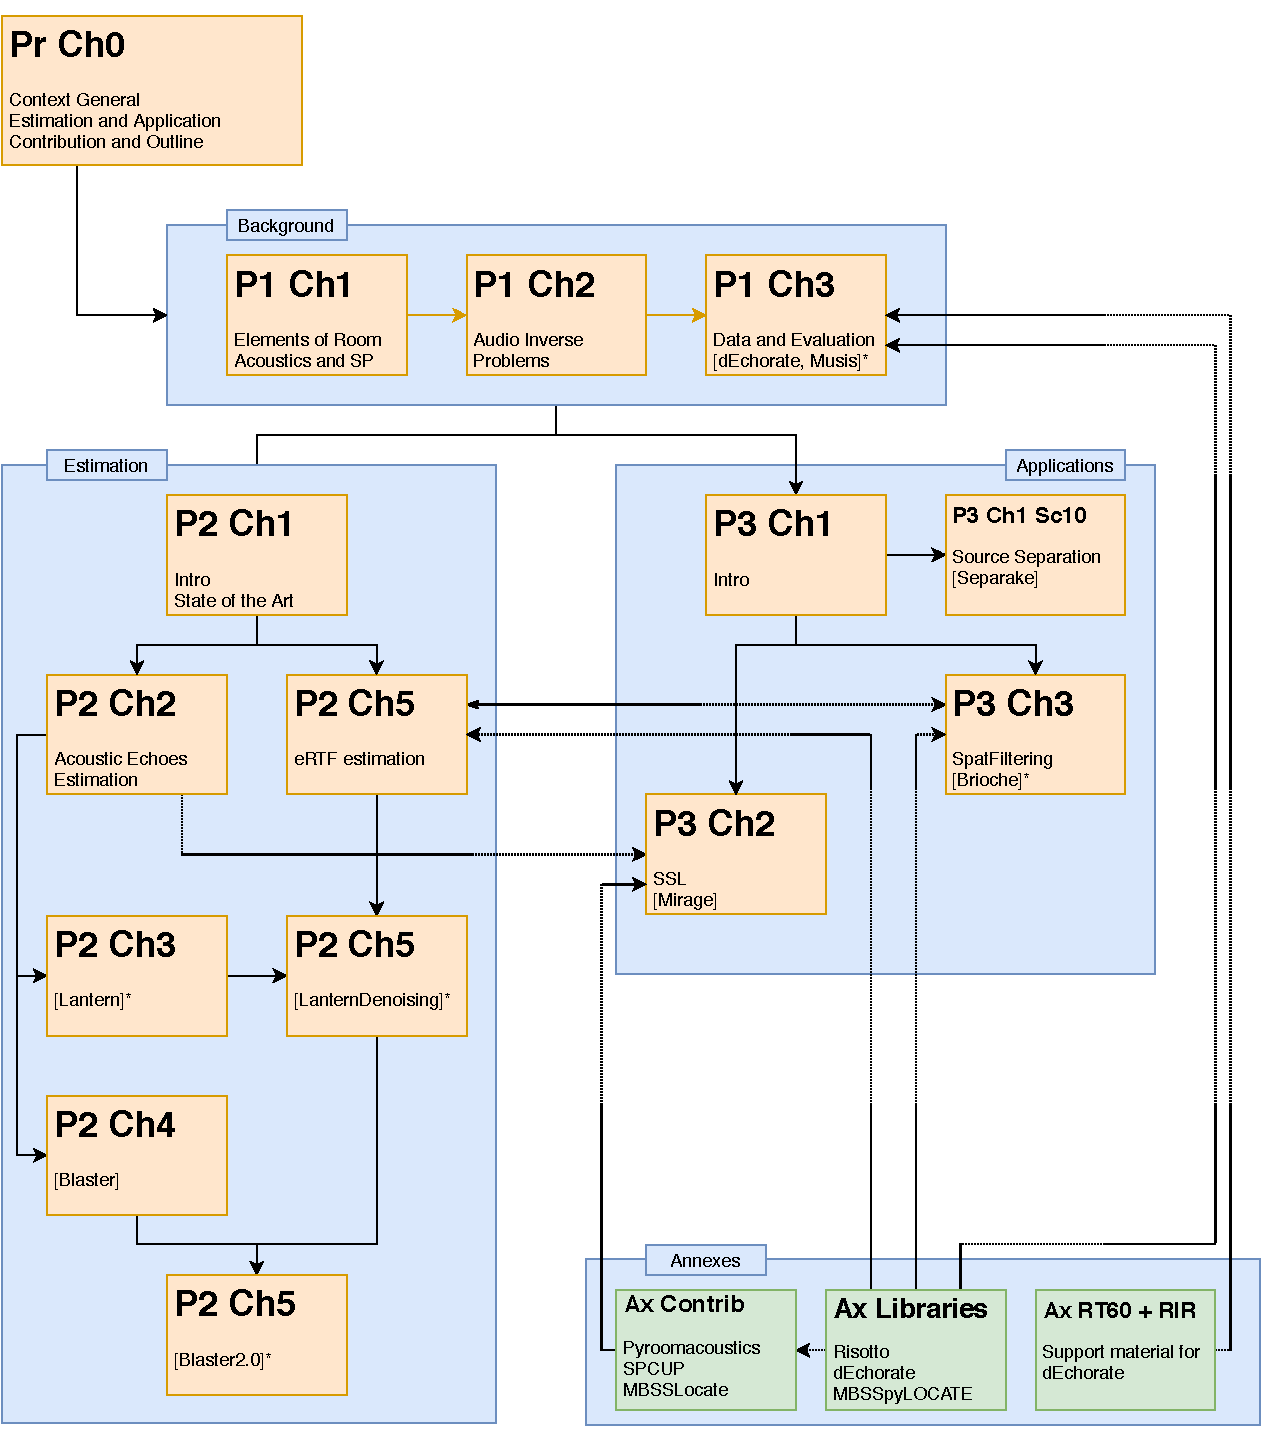
\includegraphics[width=\linewidth]{contents/assets/mindmaps/thesis_mindmap.pdf}
        \end{sidecaption}
\end{figure}

\section{Todos and Notes}

\itodo{Can we use \bison/'s argument (regarding differential cryptanalysis) for a maximal unbalanced Feistel network?}
\miss{Here something is missing}
\todo[inline]{The original todo note withouth changed colours.\newline Here's another line.}

\lipsum[11]\unsure{Is this correct?}\unsure{I'm unsure about also!}
\lipsum[11]\change{Change this!}
\lipsum[11]\info{This can help me in chapter seven!}
\lipsum[11]\plus{What was I thinking?!}
\lipsum[11]
\plus[inline]{The following section needs to be rewritten!}
\lipsum[11]

% \newthoughtpar{Incentives for new Cipher Designs}
% \blindtext

% \section{Section 1}
% \blindtext[3]

% \marginpar{%
%     \footnotesize
%     \vspace{\baselineskip}
%     \vspace*{-7\baselineskip}
%     See \cref{ch:intro} for a detailed explanation of differential cryptanalysis
%     and the problems that appear when trying to bound the differential probability.
% }

% \begin{problem}[Differentials]\label{prob:differentials}
%     \blindtext
% \end{problem}



% \section{Publications}

% During the course of my doctoral studies, I worked on several projects which are not all covered in the remainder of this thesis.
% In particular, these are the following.

% \newthoughtpar{Conference Publications}
% \begin{itemize}
% \item[] \fullfullcite{EC:CLLNW19}, see \cref{ch:bison}.
% %Because \bison/ can only be instantiated with odd block length, we here also give a second instance of the underlying construction: \wisent/.
% %This instance is for the even block length case and basically inherits almost the same security bounds as \bison/.
% \end{itemize}

% \newthoughtpar{Journal Publications}
% \begin{itemize}
%     \item[] \fullfullcite{ToSC:KraLeaWie17}.
%     \item[] \fullfullcite{ToSC:KLSW17}, see \cref{ch:slp}.
%     \item[] \fullfullcite{ToSC:LeaTezWie18}, see \cref{ch:st}.
% \end{itemize}


% \section{Stir of Echoes}

% \blindtext

% \section{Equations}

\begin{align}
    f(x) &= x^2\\
    g(x) &= \frac{1}{x}\\
    F(x) &= \int^a_b \frac{1}{3}x^3
\end{align}


A simple equation:
\[
 f(x)=(x+a)(x+b)
\]
An equation with text:
\begin{equation}
50 \text{ apples} \times 100 \text{ apples} =
\textbf{lots of apples}
\end{equation}
One including subscripts and superscripts:
\[ k_{n+1} = n^2 + k_n^2 - k_{n-1} \]
\section{Greek Letters}
\[ \alpha,  \beta,  \gamma, \Gamma, \pi, \Pi, \phi, \varphi, \mu, \Phi, \xi, \zeta \]
\[ \cos(2\theta\phi) = \cos^2 \theta\phi - \sin^2 \theta\phi \]
\section{Delimiters}
There are many types of delimiters one can use:
\[ ( a ), [ b ], \{ c \}, | d |, \| e \|,
\langle f \rangle, \lfloor g \rfloor,
\lceil h \rceil, \ulcorner i \urcorner \]
See how the delimiters are of reasonable size in these examples
\[
        \left(a+b\right)\left[1-\frac{b}{a+b}\right]=a\,,
\]
\[
        \sqrt{|xy|}\leq\left|\frac{x+y}{2}\right|,
\]
even when there is no matching delimiter
\[
        \int_a^bu\frac{d^2v}{dx^2}\,dx
        =\left.u\frac{dv}{dx}\right|_a^b
        -\int_a^b\frac{du}{dx}\frac{dv}{dx}\,dx.
\]
whereas vector problems often lead to statements such as
\[
        u=\frac{-y}{x^2+y^2}\,,\quad
        v=\frac{x}{x^2+y^2}\,,\quad\text{and}\quad
        w=0\,.
\]
\section{Multiple Fractions}
Typesetting continued fractions is easy:
\[
x = a_0 + \frac{1}{a_1 + \frac{1}{a_2 + \frac{1}{a_3 + a_4}}}
\]
However, as the fractions continue, they get smaller. If you want to keep the size consistent, use the display style; e.g.
\[
  x = a_0 + \frac{1}{\displaystyle a_1
          + \frac{1}{\displaystyle a_2
          + \frac{1}{\displaystyle a_3 + a_4}}}
\]
\section{Arrays}
Arrays of mathematics are typeset using one of the matrix environments as
in
\[
        \begin{bmatrix}
                1 & x & 0 \\
                0 & 1 & -1
        \end{bmatrix}\begin{bmatrix}
                1  \\
                y  \\
                1
        \end{bmatrix}
        =\begin{bmatrix}
                1+xy  \\
                y-1
        \end{bmatrix}.
\]
\[ \begin{pmatrix}
2 & 3 & 4\\
5 & 6 & 7\\
8 & 9 & 10 \end{pmatrix} v = 0 \]
Case statements use cases:
\[
        |x|=\begin{cases}
                x, & \text{if }x\geq 0\,,  \\
                -x, & \text{if }x< 0\,.
        \end{cases}
\]
Many arrays have lots of dots all over the place as in
\[
        \begin{matrix}
                -2 & 1 & 0 & 0 & \cdots & 0  \\
                1 & -2 & 1 & 0 & \cdots & 0  \\
                0 & 1 & -2 & 1 & \cdots & 0  \\
                0 & 0 & 1 & -2 & \ddots & \vdots \\
                \vdots & \vdots & \vdots & \ddots & \ddots & 1  \\
                0 & 0 & 0 & \cdots & 1 & -2
        \end{matrix}
\]
\section{Greek Letters}
\[ \alpha,  \beta,  \gamma, \Gamma, \pi, \Pi, \phi, \varphi, \mu, \Phi, \xi, \zeta \]
\[ \cos(2\theta\phi) = \cos^2 \theta\phi - \sin^2 \theta\phi \]
\section{Delimiters}
\[ ( a ), [ b ], \{ c \}, | d |, \| e \|,
\langle f \rangle, \lfloor g \rfloor,
\lceil h \rceil, \ulcorner i \urcorner \]
\section{Accents}
Mathematical accents are performed by a short command with one
argument, such as
\[
        \tilde f(\omega)=\frac{1}{2\pi}
        \int_{-\infty}^\infty f(x)e^{-i\omega x}\,dx\,,
\]
or
\[
        \dot{\vec \omega}=\vec r\times\vec I\,.
\]
\section{Multiline equations and aligned environments}
New lines (\\ ) do not work in equation environments. To achieve alignment of equations, use the aligned  package to produce multiline aligned math, such as:
\newline

% \[
% \begin{center}
% \begin{aligned}
% $F$ ={} & $\{F_{x} \in  F_{c} : (|S| > |C|)$ \\
%       & $\cap (\mathrm{minPixels}  < |S| < \mathrm{maxPixels})$ \\
%       & $\cap (|S_{\mathrm{conected}}| > |S| - \epsilon) $\}
% \end{aligned}
% \end{center}
% \]

% \newline

% and also:

% \newline
% \[
% \begin{center}
% \begin{aligned}
% $A_0$ & $=   \frac{1}{(\alpha+t_x)^{r+s+x}}{}_2 F_1\left( r+s+x,x+1;r+s+x+1;\frac{\alpha-\beta}{\alpha + t_x} \right) $\\
% & $\quad - \frac{1}{(\alpha+T)^{r+s+x}}{}_2 F_1\left( r+s+x,x+1;r+s+x+1;\frac{\alpha-\beta}{\alpha + T} \right),$
% \end{aligned}
% \end{center}
% \]
% \newline

\textbf{Note}: the above multiline equations have math mode defined per line, not globally at the equation level.
\section{Theorems and sets}

% \newtheorem{theorem}{Theorem}
% \newtheorem{corollary}[theorem]{Corollary}
% \newtheorem{lemma}[theorem]{Lemma}
% \newtheorem{definition}[theorem]{Definition}

\begin{theorem}
For any nonnegative integer $n$, we have
$$(1+x)^n = \sum_{i=0}^n {n \choose i} x^i$$
\end{theorem}
The Taylor series expansion for the function $e^x$ is given by
\begin{equation}
e^x = 1 + x + \frac{x^2}{2} + \frac{x^3}{6} + \cdots = \sum_{n\geq 0} \frac{x^n}{n!}
\end{equation}
\[ \forall x \in X, \quad \exists y \leq \epsilon \]
\[ \frac{n!}{k!(n-k)!} = \binom{n}{k} \]
\begin{theorem}
For any sets $A$, $B$ and $C$, we have
$$ (A\cup B)-(C-A) = A \cup (B-C)$$
\end{theorem}

\blindtext
\blinditemize

\blindtext
\blindenumerate

\blindtext
\blinddescription